\documentclass{article}
\usepackage[utf8]{inputenc}
\usepackage[margin=1in]{geometry}
\usepackage{amsmath}
\usepackage{hyperref}
\usepackage{graphicx}
\usepackage{float}
\setlength{\parindent}{0em}
\setlength{\parskip}{0.5em}

\title{CTA200 2025 Assignment 3 Submission}
\author{Sharone Abhilash}

\begin{document}

\maketitle

\section*{Question 1}

In this question, we are asked to implement an iterative function \( z_{i+1} = z_i^2 + c \), with $-2 < x < 2$ and $-2 < y < 2$. 
The function evaluates each point to determine whether the iteration remains bounded (i.e., \( |z| < 2 \)) for up to 50 steps. 
If a point diverges, it records the iteration count; otherwise, it returns \texttt{-1}.

To visualize the result, we used \texttt{matplotlib.pyplot.imshow} to display the output of the function. 
Bounded points are shown in yellow; diverged points are shown in purple using a viridis colormap:

\begin{figure}[H]
    \centering
    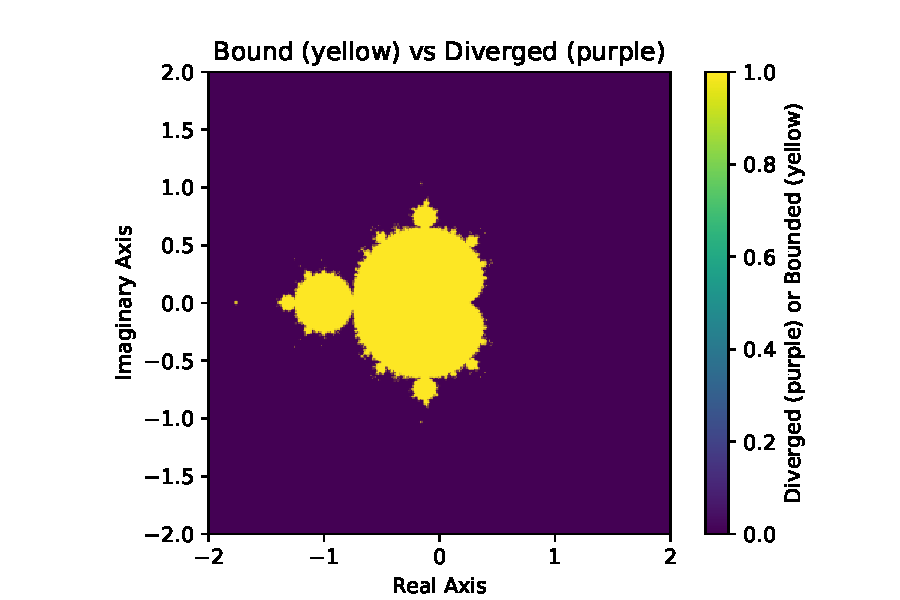
\includegraphics[width=0.6\textwidth]{question1fig1.pdf}
    \caption{Yellow regions are bounded; purple regions diverge.}
    \label{fig:q1_binary}
\end{figure}

Second, we visualize how many iterations each diverging point took. 
The slowest diverging points are near the boundary of the shape (in yellow), while the quickly diverging points appear dark more purple, and the dark purple points are points that are bound. 

\begin{figure}[H]
    \centering
    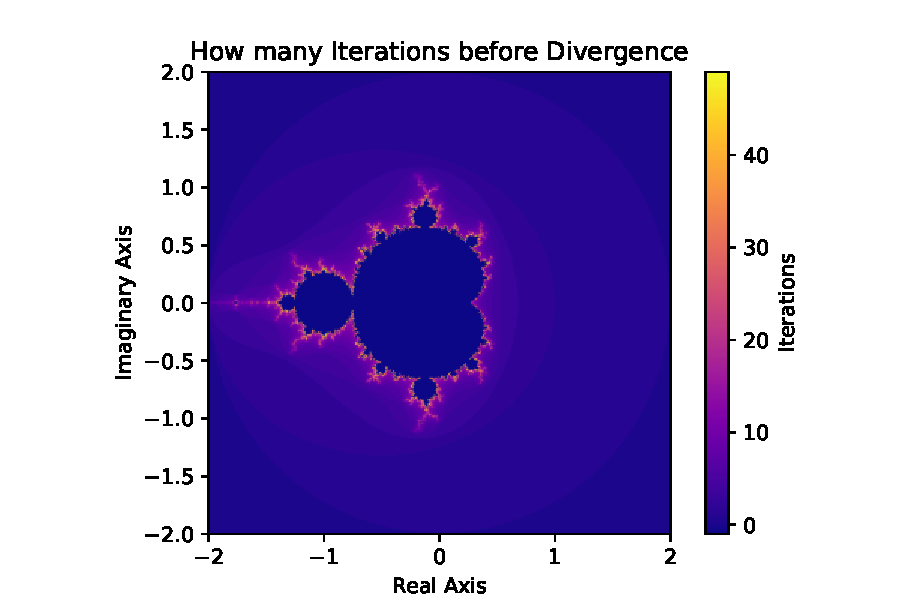
\includegraphics[width=0.6\textwidth]{question1fig2.pdf}
    \caption{Number of iterations before divergence. Brighter colors indicate slower divergence near the boundary.}
    \label{fig:q1_colored}
\end{figure}

\section*{Question 2}

The Lorenz system is a simplified model for atmospheric convection, described by the following differential equations:
\begin{eqnarray}
\dot X &=& -\sigma(X-Y)\\
\dot Y &=& rX -Y - XZ\\
\dot Z &=& -bZ + XY
\end{eqnarray}

We implemented these equations in Python, and solved them using SciPy's \texttt{solve\_ivp} 
with initial condition \( W_0 = [0., 1., 0.] \) and parameters \( \sigma = 10 \), \( r = 28 \), and \( b = 8/3 \).

We reproduced Lorenz's original Figure 1 by plotting the variable \( Y \) over three segments of 1000 iterations each.
We had a total of 3000 steps from \( t = 0 \) to \( t = 60 \).

\begin{figure}[H]
    \centering
    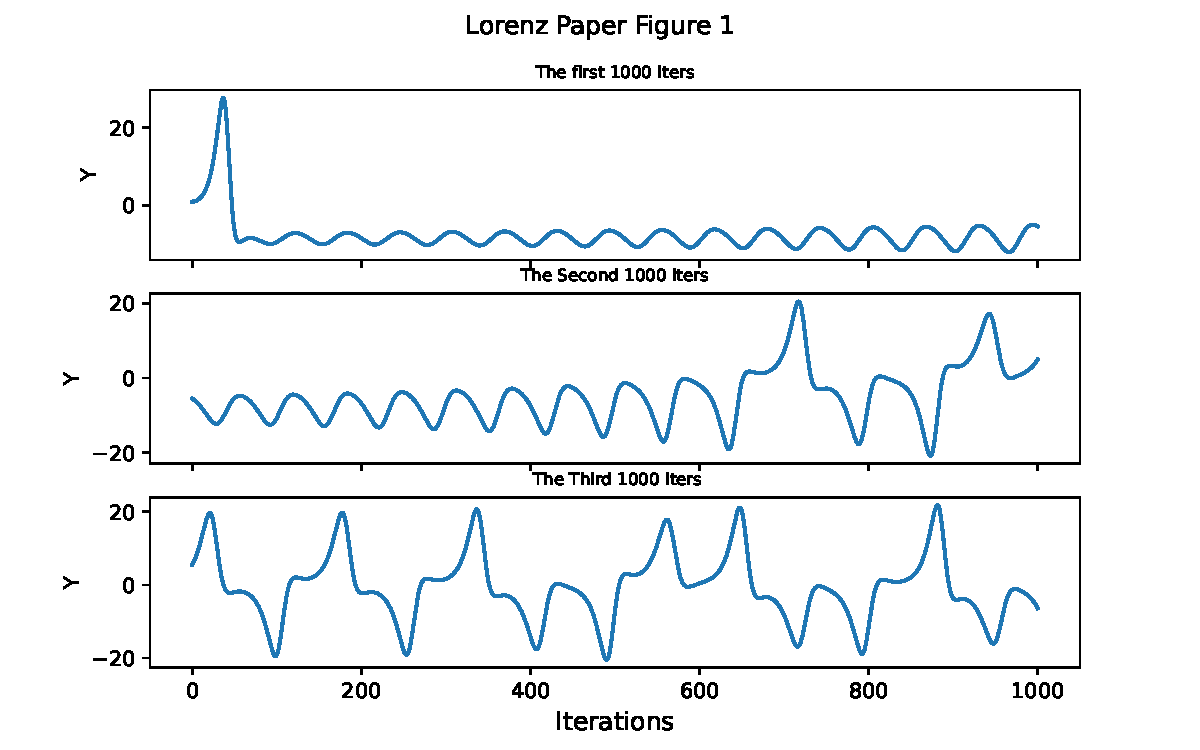
\includegraphics[width=0.6\textwidth]{question2fig1.pdf}
    \caption{\( Y \) as a function of time across three 1000-iteration segments.}
    \label{fig:q2_y_segments}
\end{figure}

Next, we show Lorenz's Figure 2 by projecting the solution from 
\( t = 14 \) to \( t = 19 \) onto the \( X\text{-}Y \) and \( Y\text{-}Z \) planes.
The solution is first evaluated from \( t = 0\) to \( t = 14 \), and that final state is used as the initial condition for the solution until \( t = 19 \). 

\begin{figure}[H]
    \centering
    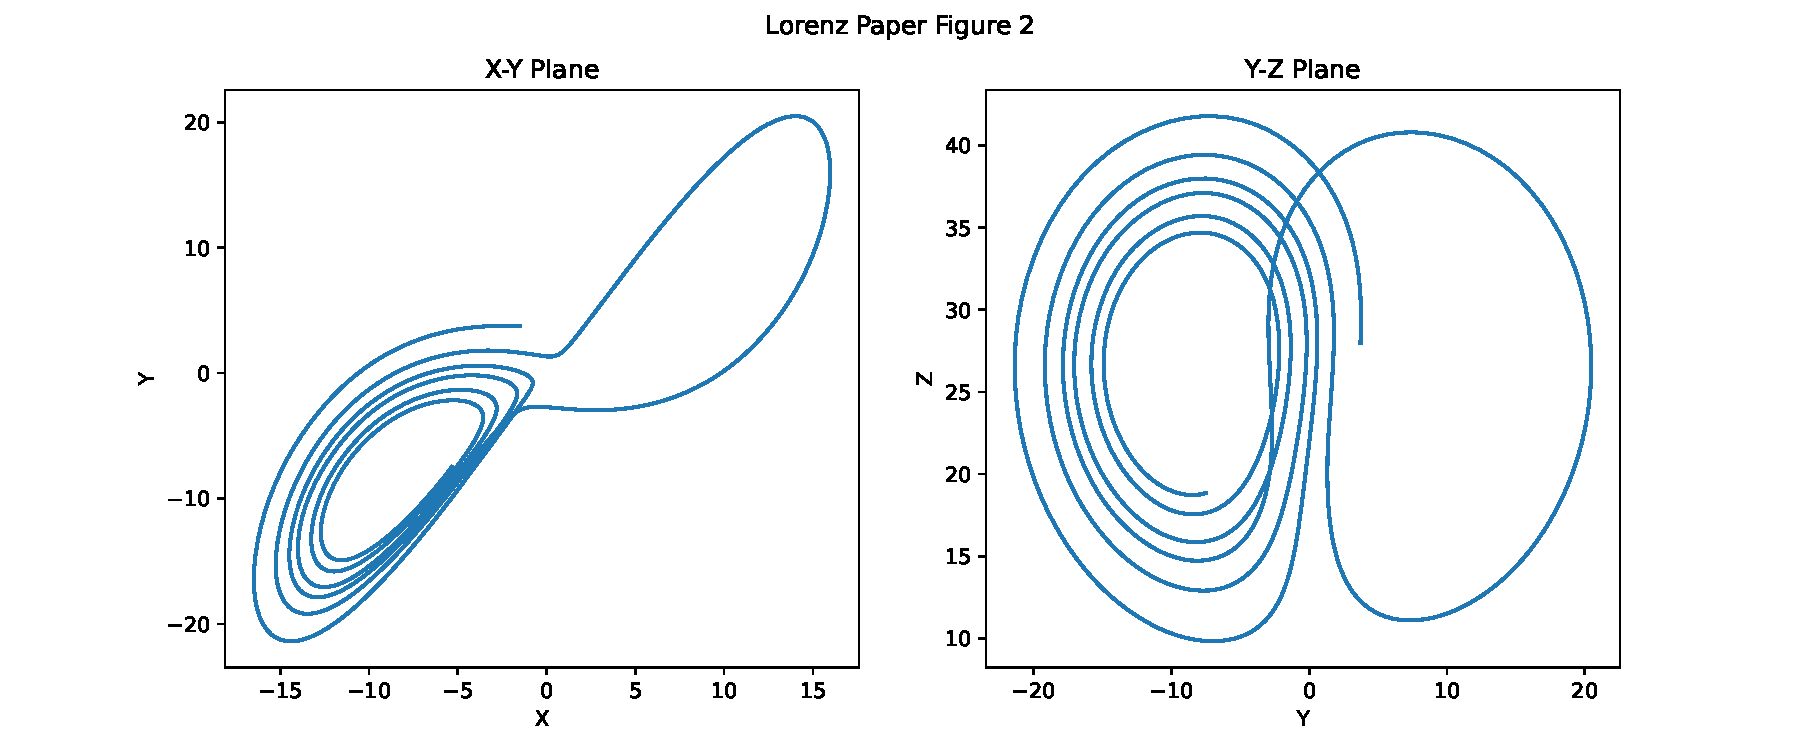
\includegraphics[width=0.9\textwidth]{question2fig2.pdf}
    \caption{Phase space projections: Left is the \( X\text{-}Y \) plane, right is the \( Y\text{-}Z \) plane.}
    \label{fig:q2_phase}
\end{figure}

Finally, we also note that the Lorenz system can become unpredictable even if the initial conditions change slightly. 
We solved it again with a slightly changed initial condition \( W_0' = [0., 1.00000001, 0.] \), and computed the distance between the original and perturbed solutions at each time step.

\begin{figure}[H]
    \centering
    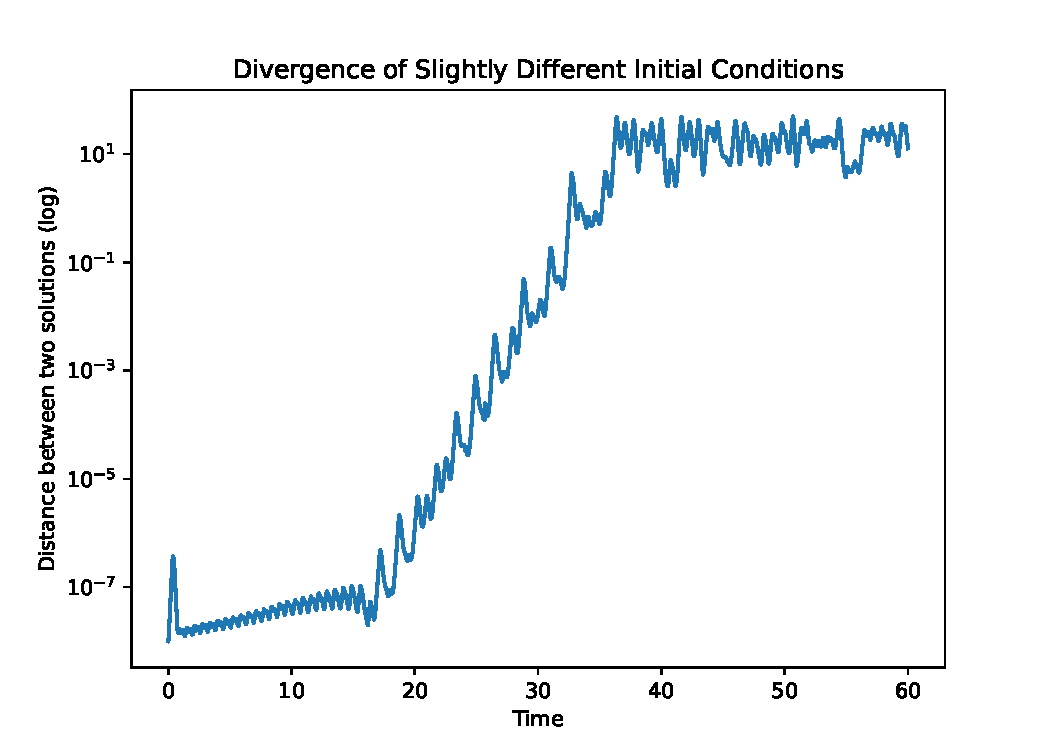
\includegraphics[width=0.6\textwidth]{question2fig3.pdf}
    \caption{Log-scale plot of distance between two solutions with slightly different initial conditions.}
    \label{fig:q2_divergence}
\end{figure}

\end{document}
